\documentclass{standalone}
\usepackage{tikz}
\usetikzlibrary{patterns, positioning}

\begin{document}
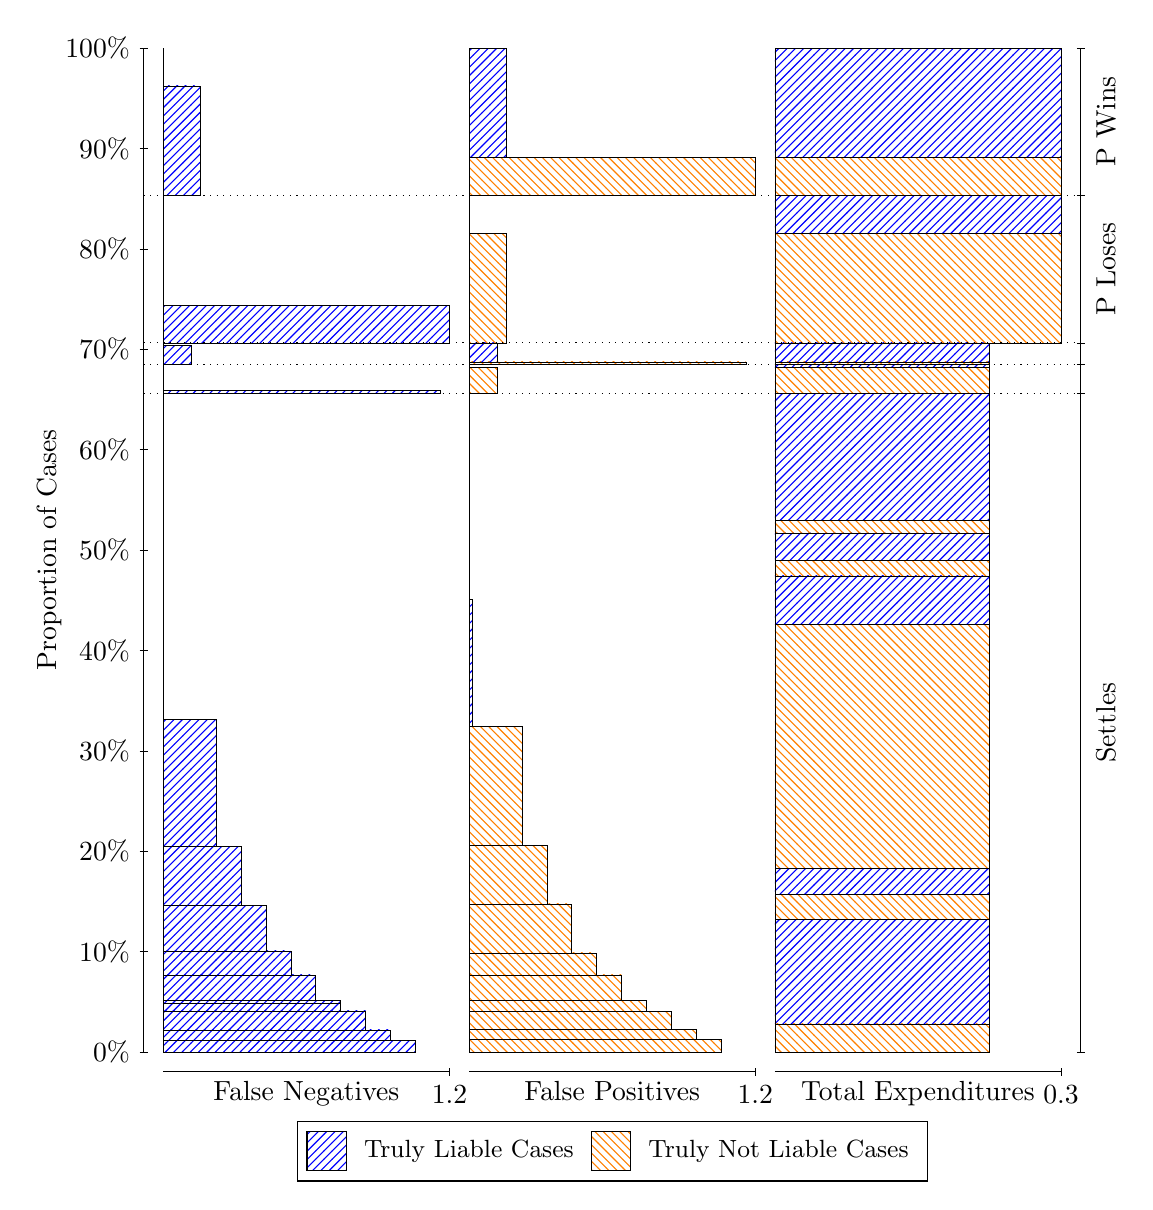
\begin{tikzpicture}
\draw[black, very thin] (1.5,1.75) -- (1.5,14.5);
\node[rotate=90, anchor=center] at (0.3, 8.125) {Proportion of Cases};
\draw[black, very thin] (1.45,1.75) -- (1.55,1.75);
\node[anchor=east] at (1.45, 1.75) {0\%};
\draw[black, very thin] (1.45,3.025) -- (1.55,3.025);
\node[anchor=east] at (1.45, 3.025) {10\%};
\draw[black, very thin] (1.45,4.3) -- (1.55,4.3);
\node[anchor=east] at (1.45, 4.3) {20\%};
\draw[black, very thin] (1.45,5.575) -- (1.55,5.575);
\node[anchor=east] at (1.45, 5.575) {30\%};
\draw[black, very thin] (1.45,6.85) -- (1.55,6.85);
\node[anchor=east] at (1.45, 6.85) {40\%};
\draw[black, very thin] (1.45,8.125) -- (1.55,8.125);
\node[anchor=east] at (1.45, 8.125) {50\%};
\draw[black, very thin] (1.45,9.4) -- (1.55,9.4);
\node[anchor=east] at (1.45, 9.4) {60\%};
\draw[black, very thin] (1.45,10.675) -- (1.55,10.675);
\node[anchor=east] at (1.45, 10.675) {70\%};
\draw[black, very thin] (1.45,11.95) -- (1.55,11.95);
\node[anchor=east] at (1.45, 11.95) {80\%};
\draw[black, very thin] (1.45,13.225) -- (1.55,13.225);
\node[anchor=east] at (1.45, 13.225) {90\%};
\draw[black, very thin] (1.45,14.5) -- (1.55,14.5);
\node[anchor=east] at (1.45, 14.5) {100\%};

\draw[black, very thin] (13.4,1.75) -- (13.4,14.5);
\draw[black, very thin] (13.35,1.75) -- (13.45,1.75);
\node[anchor=west] at (13.35, 1.75) {};
\draw[black, very thin] (13.35,10.113) -- (13.45,10.113);
\node[anchor=west] at (13.35, 10.113) {};
\draw[black, very thin] (13.35,10.484) -- (13.45,10.484);
\node[anchor=west] at (13.35, 10.484) {};
\draw[black, very thin] (13.35,10.755) -- (13.45,10.755);
\node[anchor=west] at (13.35, 10.755) {};
\draw[black, very thin] (13.35,12.629) -- (13.45,12.629);
\node[anchor=west] at (13.35, 12.629) {};
\draw[black, very thin] (13.35,14.5) -- (13.45,14.5);
\node[anchor=west] at (13.35, 14.5) {};

\draw[black, very thin, pattern color=blue, pattern=north east lines] (1.75,1.75) rectangle (4.9489,1.8957);
\draw[black, very thin, pattern color=blue, pattern=north east lines] (1.75,1.8957) rectangle (4.633,2.0294);
\draw[black, very thin, pattern color=blue, pattern=north east lines] (1.75,2.0294) rectangle (4.317,2.272);
\draw[black, very thin, pattern color=blue, pattern=north east lines] (1.75,2.272) rectangle (4.0011,2.3658);
\draw[black, very thin, pattern color=blue, pattern=north east lines] (1.75,2.3658) rectangle (4.0011,2.4068);
\draw[black, very thin, pattern color=blue, pattern=north east lines] (1.75,2.4068) rectangle (3.6851,2.7296);
\draw[black, very thin, pattern color=blue, pattern=north east lines] (1.75,2.7296) rectangle (3.3692,3.0346);
\draw[black, very thin, pattern color=blue, pattern=north east lines] (1.75,3.0346) rectangle (3.0533,3.6069);
\draw[black, very thin, pattern color=blue, pattern=north east lines] (1.75,3.6069) rectangle (2.7373,4.3619);
\draw[black, very thin, pattern color=blue, pattern=north east lines] (1.75,4.3619) rectangle (2.4214,5.975);
\draw[black, very thin, pattern color=orange, pattern=north west lines] (1.75,5.975) rectangle (1.75,10.113);
\draw[black, very thin, pattern color=blue, pattern=north east lines] (1.75,10.113) rectangle (5.2649,10.151);
\draw[black, very thin, pattern color=orange, pattern=north west lines] (1.75,10.151) rectangle (1.75,10.484);
\draw[black, very thin, pattern color=blue, pattern=north east lines] (1.75,10.484) rectangle (2.1054,10.725);
\draw[black, very thin, pattern color=orange, pattern=north west lines] (1.75,10.725) rectangle (1.75,10.755);
\draw[black, very thin, pattern color=blue, pattern=north east lines] (1.75,10.755) rectangle (5.3833,11.236);
\draw[black, very thin, pattern color=orange, pattern=north west lines] (1.75,11.236) rectangle (1.75,12.629);
\draw[black, very thin, pattern color=blue, pattern=north east lines] (1.75,12.629) rectangle (2.2239,14.018);
\draw[black, very thin, pattern color=orange, pattern=north west lines] (1.75,14.018) rectangle (1.75,14.5);
\draw[black, very thin, pattern color=orange, pattern=north west lines] (5.6333,1.75) rectangle (8.8322,1.9061);
\draw[black, very thin, pattern color=orange, pattern=north west lines] (5.6333,1.9061) rectangle (8.5163,2.0405);
\draw[black, very thin, pattern color=orange, pattern=north west lines] (5.6333,2.0405) rectangle (8.2004,2.2623);
\draw[black, very thin, pattern color=orange, pattern=north west lines] (5.6333,2.2623) rectangle (7.8844,2.4078);
\draw[black, very thin, pattern color=orange, pattern=north west lines] (5.6333,2.4078) rectangle (7.5685,2.729);
\draw[black, very thin, pattern color=orange, pattern=north west lines] (5.6333,2.729) rectangle (7.2525,3.0074);
\draw[black, very thin, pattern color=orange, pattern=north west lines] (5.6333,3.0074) rectangle (6.9366,3.6304);
\draw[black, very thin, pattern color=orange, pattern=north west lines] (5.6333,3.6304) rectangle (6.6207,4.3759);
\draw[black, very thin, pattern color=orange, pattern=north west lines] (5.6333,4.3759) rectangle (6.3047,5.8879);
\draw[black, very thin, pattern color=blue, pattern=north east lines] (5.6333,5.8879) rectangle (5.6728,7.501);
\draw[black, very thin, pattern color=blue, pattern=north east lines] (5.6333,7.501) rectangle (5.6333,10.113);
\draw[black, very thin, pattern color=orange, pattern=north west lines] (5.6333,10.113) rectangle (5.9888,10.446);
\draw[black, very thin, pattern color=blue, pattern=north east lines] (5.6333,10.446) rectangle (5.6333,10.484);
\draw[black, very thin, pattern color=orange, pattern=north west lines] (5.6333,10.484) rectangle (9.1482,10.514);
\draw[black, very thin, pattern color=blue, pattern=north east lines] (5.6333,10.514) rectangle (5.9888,10.755);
\draw[black, very thin, pattern color=orange, pattern=north west lines] (5.6333,10.755) rectangle (6.1072,12.148);
\draw[black, very thin, pattern color=blue, pattern=north east lines] (5.6333,12.148) rectangle (5.6333,12.629);
\draw[black, very thin, pattern color=orange, pattern=north west lines] (5.6333,12.629) rectangle (9.2667,13.111);
\draw[black, very thin, pattern color=blue, pattern=north east lines] (5.6333,13.111) rectangle (6.1072,14.5);
\draw[black, very thin, pattern color=orange, pattern=north west lines] (9.5167,1.75) rectangle (12.242,2.1063);
\draw[black, very thin, pattern color=blue, pattern=north east lines] (9.5167,2.1063) rectangle (12.242,3.4335);
\draw[black, very thin, pattern color=orange, pattern=north west lines] (9.5167,3.4335) rectangle (12.242,3.7547);
\draw[black, very thin, pattern color=blue, pattern=north east lines] (9.5167,3.7547) rectangle (12.242,4.0775);
\draw[black, very thin, pattern color=orange, pattern=north west lines] (9.5167,4.0775) rectangle (12.242,7.1807);
\draw[black, very thin, pattern color=blue, pattern=north east lines] (9.5167,7.1807) rectangle (12.242,7.7965);
\draw[black, very thin, pattern color=orange, pattern=north west lines] (9.5167,7.7965) rectangle (12.242,7.9977);
\draw[black, very thin, pattern color=blue, pattern=north east lines] (9.5167,7.9977) rectangle (12.242,8.3437);
\draw[black, very thin, pattern color=orange, pattern=north west lines] (9.5167,8.3437) rectangle (12.242,8.4998);
\draw[black, very thin, pattern color=blue, pattern=north east lines] (9.5167,8.4998) rectangle (12.242,10.113);
\draw[black, very thin, pattern color=orange, pattern=north west lines] (9.5167,10.113) rectangle (12.242,10.446);
\draw[black, very thin, pattern color=blue, pattern=north east lines] (9.5167,10.446) rectangle (12.242,10.484);
\draw[black, very thin, pattern color=orange, pattern=north west lines] (9.5167,10.484) rectangle (12.242,10.514);
\draw[black, very thin, pattern color=blue, pattern=north east lines] (9.5167,10.514) rectangle (12.242,10.755);
\draw[black, very thin, pattern color=orange, pattern=north west lines] (9.5167,10.755) rectangle (13.15,12.148);
\draw[black, very thin, pattern color=blue, pattern=north east lines] (9.5167,12.148) rectangle (13.15,12.629);
\draw[black, very thin, pattern color=orange, pattern=north west lines] (9.5167,12.629) rectangle (13.15,13.111);
\draw[black, very thin, pattern color=blue, pattern=north east lines] (9.5167,13.111) rectangle (13.15,14.5);
\draw[black, dotted] (1.5,10.113) -- (13.4,10.113);
\draw[black, dotted] (1.5,10.484) -- (13.4,10.484);
\draw[black, dotted] (1.5,10.755) -- (13.4,10.755);
\draw[black, dotted] (1.5,12.629) -- (13.4,12.629);
\draw[black, very thin] (1.75,1.5) -- (5.3833,1.5);
\node[anchor=north] at (3.5667, 1.5) {False Negatives};
\draw[black, very thin] (5.3833,1.45) -- (5.3833,1.55);
\node[anchor=north] at (5.3833, 1.45) {1.2};

\draw[black, very thin] (5.6333,1.5) -- (9.2667,1.5);
\node[anchor=north] at (7.45, 1.5) {False Positives};
\draw[black, very thin] (9.2667,1.45) -- (9.2667,1.55);
\node[anchor=north] at (9.2667, 1.45) {1.2};

\draw[black, very thin] (9.5167,1.5) -- (13.15,1.5);
\node[anchor=north] at (11.333, 1.5) {Total Expenditures};
\draw[black, very thin] (13.15,1.45) -- (13.15,1.55);
\node[anchor=north] at (13.15, 1.45) {0.3};

\node[black, centered, rotate=90] at (13.72, 5.9314) {Settles};


\node[black, centered, rotate=90] at (13.72, 11.692) {P Loses};
\node[black, centered, rotate=90] at (13.72, 13.565) {P Wins};

\draw (7.449999999999999,1.5) node[draw=none] (baseCoordinate) {};
\begin{scope}[align=center]
        \matrix[scale=0.5, draw=black, below=0.5cm of baseCoordinate, nodes={draw}, column sep=0.1cm]{
            \node[rectangle, draw, minimum width=0.5cm, minimum height=0.5cm, pattern=north east lines, pattern color=blue] {}; &
            \node[draw=none, font=\small] (B) {Truly Liable Cases}; &
            \node[rectangle, draw, minimum width=0.5cm, minimum height=0.5cm, pattern=north west lines, pattern color=orange] {}; &
            \node[draw=none, font=\small] (B) {Truly Not Liable Cases}; \\
            };
\end{scope}

\end{tikzpicture}
\end{document}